In software development a process model is organizational framework that describes the way in which the software is developed. It defines different phases of the development, activities that are carried out during these phases, rules and criteria for advancing of phases and different roles for the team members. For this project an iterative waterfall-model was chosen as development process. 
The regular waterfall model is defines as shown in Figure \ref{waterfall}. The development phases shown in the figure are strictly executed one after the other, as each of them depend on the result of the previous ones. \\ In every iterative development-model, the desired functionality of the product is divided into smaller parts that can be implemented independently. In every development cycle new system elements are added, thus reducing the  complexity of each cycle.\\ In the iterative waterfall model the simple waterfall model is used for each of these iterations. \\ The main advantages of this approach are:
\begin{itemize}
\item Reduced complexity of the individual development steps
\item Continuous feasibility and success checking with the end of each iteration
\item Development cycles of system parts with lose coupling can be carried out simultaneously
\end{itemize}
As code and revision management tool git is used, the repository is hosted at github: \url{http://github.com/mrtazz/kangaroo/}
\begin{figure}[h!]
\centering
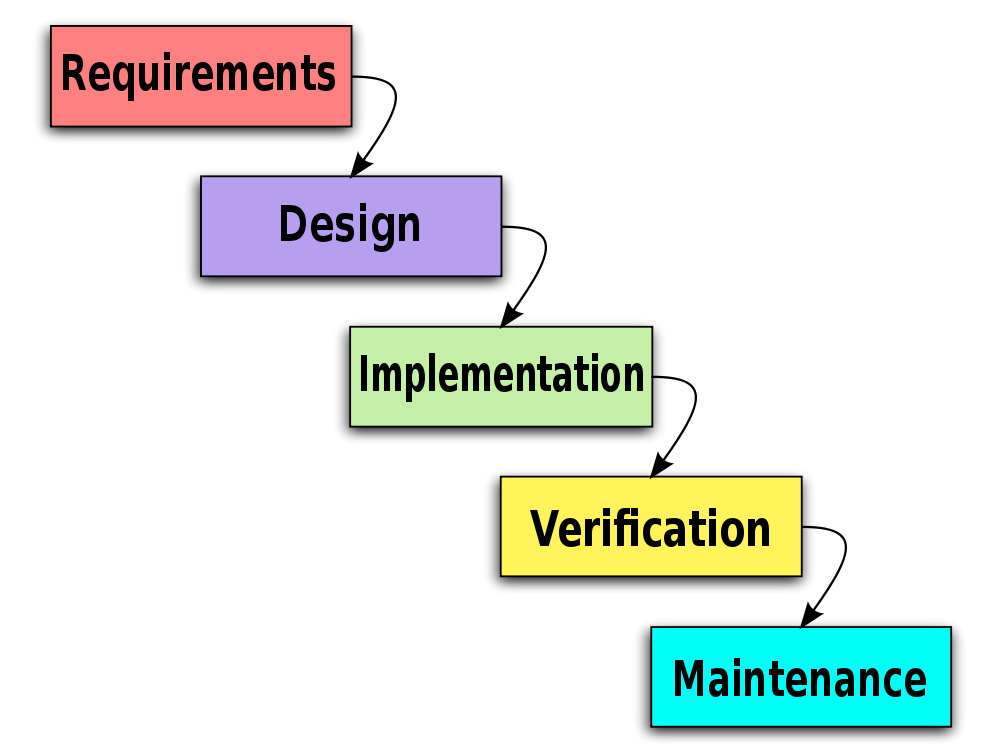
\includegraphics[width=14cm]{pics/waterfall.png}
\caption{Generic waterfall model}
\label{waterfall}
\end{figure}  


